\scanpage{18}
\uline{Interprétations en termes de filtrations du foncteur oubli \deleted{sur la catégorie}} des représentations linéaires de dimension finie de $G$. (Il s'agit de
% Typed interlinear addition, with its joined curved enclosure and descending leader.
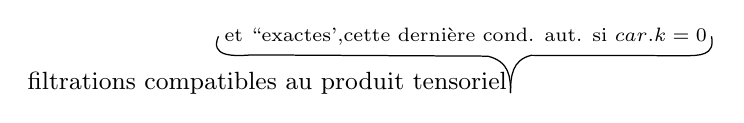
\begin{tikzpicture}[baseline=(body.base),inner sep=0pt,x=1cm,y=1cm]
\node[anchor=base west,font=\small] (body) at (0,0) {filtrations compatibles au produit tensoriel};
\node[anchor=base west,font=\scriptsize] (add) at (2.5,.62) {\inserted{et ``exactes',cette \unsure{dernière} cond. aut. si $\operatorname{car}.k=0$}};
\draw[line width=.45pt] ([xshift=-.07cm]add.west) .. controls ([xshift=-.18cm,yshift=-.14cm]add.south west) and ([xshift=.1cm,yshift=-.14cm]add.south west) .. ([xshift=.35cm,yshift=-.12cm]add.south west) -- ([xshift=-.25cm,yshift=.35cm]body.east) .. controls ([xshift=.03cm,yshift=.28cm]body.east) and ([xshift=.04cm,yshift=.08cm]body.east) .. ([xshift=.04cm,yshift=-.12cm]body.east);
\draw[line width=.45pt] ([xshift=.05cm]add.east) .. controls ([xshift=.1cm,yshift=-.13cm]add.south east) and ([xshift=-.1cm,yshift=-.13cm]add.south east) .. ([xshift=-.3cm,yshift=-.13cm]add.south east) -- ([xshift=.3cm,yshift=.36cm]body.east) .. controls ([xshift=.06cm,yshift=.3cm]body.east) and ([xshift=.04cm,yshift=.1cm]body.east) .. ([xshift=.04cm,yshift=-.12cm]body.east);
\end{tikzpicture}). Supposons fixé une classe
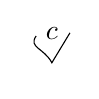
\begin{tikzpicture}[baseline=(base.base),inner sep=0pt]
\node (base) at (0,0) {\phantom{$c$}};
\node at (0,.4) {\inserted{\handwritten{$c$}}};
\draw (-.2,.37) .. controls (-.3,.22) and (-.1,.22) .. (0,.03) -- (.23,.41);
\end{tikzpicture}
de
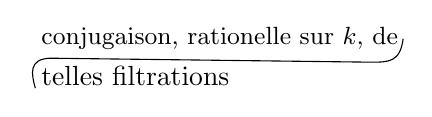
\begin{tikzpicture}[baseline=(base.base),inner sep=0pt,x=1cm,y=1cm]
\node[anchor=base west] (base) at (0,0) {telles filtrations};
\node[anchor=base west,font=\small] (add) at (0,.52) {\inserted{conjugaison, rationelle sur $k$, de}};
\draw ([xshift=.06cm]add.east) .. controls ([xshift=.02cm,yshift=-.15cm]add.south east) and ([xshift=-.12cm,yshift=-.15cm]add.south east) .. ([xshift=-.35cm,yshift=-.15cm]add.south east) -- ([xshift=.12cm,yshift=.23cm]base.west) .. controls ([xshift=-.16cm,yshift=.22cm]base.west) and ([xshift=-.12cm,yshift=.03cm]base.west) .. ([xshift=-.07cm,yshift=-.15cm]base.west);
\end{tikzpicture}
(NB elle n'admet pas nécessairement un représentant rat/$k$); 
% Both o and l contours survive in the second cell; no chronological ordering is assigned.
i\unsure{
\begin{tikzpicture}[baseline=(ol.base),inner sep=0pt]
\node (ol) at (0,0) {o};\node at (0,.01) {l};
\end{tikzpicture}}\deleted{\unsure{n}} revient au même de se donner,\deleted{un} pour le Chevalley $G_o$ associé à $G$, un \deleted{homomorphisme} élément de $\operatorname{Hom}(\underline{G}_m,T_o)/W=M/W$ ($T_o=M\mathbin{\text{\textcircled{x}}}\underline{G}_m$ est le tore maximal type de $G_o$) invariant par le sous-groupe
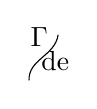
\begin{tikzpicture}[baseline=(base.base),inner sep=0pt]
\node[anchor=base west] (base) at (0,0) {de};
\node at (-.02,.43) {\inserted{\handwritten{$\Gamma$}}};
\draw (-.15,-.12) .. controls (-.16,.15) and (.18,.19) .. (.22,.46);
\end{tikzpicture}
$\operatorname{Auext}G_o=E_o$ image de $\operatorname{Gal}(\handwritten{\bar{k}}/k)$, ou encore un \deleted{homomorphisme $\underline{G}_m\unsure{\to}T$} élément de $M$ qui soit dans la chambre de Weyl de $M\mathbin{\text{\textcircled{x}}}_{\underline{Z}}\underline{R}$ et qui soit stable par $\handwritten{\Gamma}$. On a alors le \unsure{schéma} $\handwritten{\underline{
\begin{tikzpicture}[baseline=-.15ex,x=1ex,y=1ex]\draw[line width=.35pt] (.42,.53) ellipse (.32 and .46);\draw[line width=.35pt] (-.02,-.16)--(.84,1.27);\end{tikzpicture}}_c}$ des filtrations de classe $\handwritten{c}$, qui est un espace homogène sous $G$, de
% The long insertion's enclosure bends down immediately after paraboliques;.
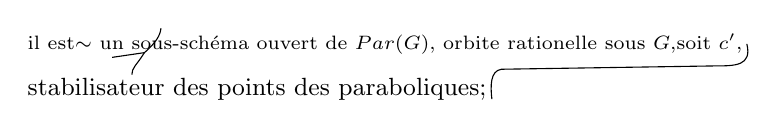
\begin{tikzpicture}[baseline=(base.base),inner sep=0pt,x=1cm,y=1cm]
\node[anchor=base west,font=\small] (base) at (0,0) {stabilisateur des points des paraboliques;};
\node[anchor=base west,font=\scriptsize] (add) at (0,.59) {\inserted{\handwritten{il} est\inserted{\handwritten{$\sim$}} un sous-schéma ouvert de $\uline{Par}(G)$, orbite rationelle sous $G$,\handwritten{soit $c'$,}}};
\draw ([xshift=.05cm]add.east) .. controls ([xshift=.12cm,yshift=-.14cm]add.south east) and ([xshift=-.1cm,yshift=-.14cm]add.south east) .. ([xshift=-.35cm,yshift=-.14cm]add.south east) -- ([xshift=.18cm,yshift=.26cm]base.east) .. controls ([xshift=.04cm,yshift=.24cm]base.east) and ([xshift=.04cm,yshift=.05cm]base.east) .. ([xshift=.06cm,yshift=-.12cm]base.east);
% A second, small curved leader accompanies the raised similarity sign.
\draw (1.08,.49) -- (1.49,.55) .. controls (1.64,.68) and (1.69,.77) .. (1.7,.86);
\draw (1.49,.55) .. controls (1.39,.39) and (1.33,.36) .. (1.33,.27);
\end{tikzpicture}
On peut regarder aussi le schéma $\operatorname{ST}_c$ des homomorphismes $i:\underline{G}_m\handwritten{\to}G$ de classe $c$, qui est donc une orbite rationelle de $G$ opérant sur $\uline{Homgr}(\underline{G}_m,G)$. Il est canoniquement isomorphe au schéma des couples de Lévi $(P,L)$ tels que $P$ soit de classe $c'$. (En d'autres termes, grâce au choix d'un $c$, pour $P$\inserted{\begin{tikzpicture}[baseline=(attach)]
  \node[anchor=west,inner sep=0pt] at (0,.34) {ou encore $\handwritten{\underline{\begin{tikzpicture}[baseline=-.15ex,x=1ex,y=1ex]\draw[line width=.35pt] (.42,.53) ellipse (.32 and .46);\draw[line width=.35pt] (-.02,-.16)--(.84,1.27);\end{tikzpicture}}}$};
  \coordinate (attach) at (-.06,-.15);
  \draw[gray,line width=.25pt] (-.15,-.29) .. controls (-.12,.08) and (.03,.08) .. (.21,.08) -- (2.45,.13) .. controls (2.59,.13) and (2.73,.22) .. (2.78,.43);
  \draw[line width=.5pt] (attach) .. controls (-.06,.16) and (.05,.14) .. (.25,.14) -- (2.84,.14) .. controls (2.98,.14) and (2.99,.23) .. (2.99,.39);
\end{tikzpicture}} de classe $c'$ donné,
il revient au même de se donner un $i:\underline{G}_m\handwritten{\to}P$ de la classe définie par $c$, où un sous-groupe de Lévi de $P$, à $i$ étant associé \unsure{\tikz[baseline=-.45ex]{\fill[rotate=-35] (0,0) ellipse (.35pt and .65pt);}} $\operatorname{Cent}(i)$.\handwritten{)} On a 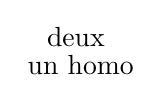
\begin{tikzpicture}[baseline=(old.base),x=1em,y=1em]
\node[anchor=base west,inner sep=0pt] (old) at (0,0) {\deleted{un homo}};
\node[anchor=base west,inner sep=0pt] at (.7,1) {\inserted{deux}};
\end{tikzpicture}morphismesde schémas canoniquement isomorphes
\[
\operatorname{ST}_c\handwritten{\longrightarrow\underline{
\begin{tikzpicture}[baseline=-.15ex,x=1ex,y=1ex]\draw[line width=.35pt] (.42,.53) ellipse (.32 and .46);\draw[line width=.35pt] (-.02,-.16)--(.84,1.27);\end{tikzpicture}}}_c\quad,\quad
(\operatorname{CL})_{c'}\handwritten{\longrightarrow}\operatorname{Par}_{c'}\quad,
\]
le premier en termes de théorie des filtrations d\unsure{%

\begin{tikzpicture}[baseline=(a.base)]
\node[inner sep=0pt] (a) at (0,0) {a};
\node[inner sep=0pt] at (-.015em,.025em) {e};
\end{tikzpicture}} foncteurs fibres, le deuxième \deleted{d}en termes de groupes paraboliques.

Supposons maintenant que $k$ soit de car. nulle (j'ignore dans quelle mesure c'est vraiment nécessaire). On peut alors considérer le Schéma $\operatorname{Dyn}_c$ des homomorphismes $f:\operatorname{Sl}(2,k)\handwritten{\longrightarrow}G$ tels que $fi_o$ soit de classe $c$. Supposons-le
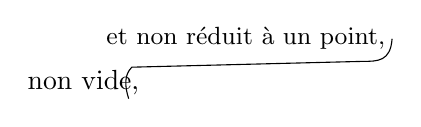
\begin{tikzpicture}[baseline=(base.base),inner sep=0pt,x=1cm,y=1cm]
\node[anchor=base west] (base) at (0,0) {non vide,};
\node[anchor=base west,font=\small] (add) at (1,.56) {\inserted{\handwritten{et non réduit à un point,}}};
\draw ([xshift=.08cm]add.east) .. controls ([xshift=.06cm,yshift=-.14cm]add.south east) and ([xshift=-.1cm,yshift=-.14cm]add.south east) .. ([xshift=-.3cm,yshift=-.14cm]add.south east) -- ([xshift=-.1cm,yshift=.19cm]base.east) .. controls ([xshift=-.2cm,yshift=.09cm]base.east) and ([xshift=-.19cm,yshift=-.05cm]base.east) .. ([xshift=-.14cm,yshift=-.21cm]base.east);
\end{tikzpicture}
i.e. $c$ une classe de
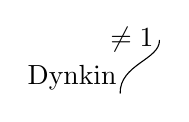
\begin{tikzpicture}[baseline=(base.base),inner sep=0pt]
\node[anchor=base west] (base) at (0,0) {Dynkin};
\node[anchor=base west] (add) at (1.05,.48) {\inserted{\handwritten{$\ne1$}}};
\draw ([xshift=.07cm]add.east) .. controls ([xshift=.08cm,yshift=-.25cm]add.east) and ([xshift=.03cm,yshift=.17cm]base.east) .. ([xshift=.04cm,yshift=-.2cm]base.east);
\end{tikzpicture}.
Alors $\operatorname{Dyn}_c$ est un \deleted{\uline{torseur}}\inserted{\handwritten{espace homogène}} sous $G$
\inserted{\handwritten{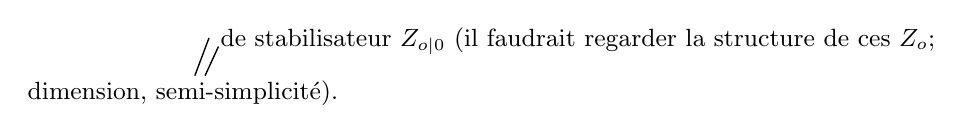
\begin{tikzpicture}[baseline=(attach)]
  \node[anchor=west,inner sep=0pt,font=\small] at (0,.42) {de stabilisateur $Z_{\unsure{o|0}}$ (il faudrait regarder la structure de ces $Z_o$;};
  \node[anchor=west,inner sep=0pt,font=\small] at (-2.45,-.24) {dimension, semi-simplicité).};
  \coordinate (attach) at (-.25,0);
  \draw[line width=.5pt] (-.32,-.02) -- (-.14,.46);
  \draw[line width=.5pt] (-.19,-.02) -- (-.02,.35);
\end{tikzpicture}}}\deleted{(en fait, il est can. is. au torseur $\uline{Isom}(G_1,G)$, où $G_1$ est le groupe quasi-déployé correspondant à $G$).} Soit $\operatorname{Un}_c$ le schéma des éléments
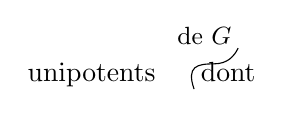
\begin{tikzpicture}[baseline=(base.base),inner sep=0pt,x=1cm,y=1cm]
\node[anchor=base west] (base) at (0,0) {unipotents};
\node[anchor=base west] (tail) at (2.2,0) {dont};
\node[anchor=base west,font=\small] (add) at (1.9,.46) {\inserted{\handwritten{de $G$}}};
\draw (2.12,-.1) .. controls (2.02,.19) and (2.16,.22) .. (2.37,.22) .. controls (2.55,.22) and (2.63,.32) .. (2.68,.42);
\end{tikzpicture}
la classe corresponde à \deleted{celle de} $c$ par la correspondance
% archive sheet number: 17
